\documentclass[11pt]{article}
\usepackage[T1]{fontenc}
\usepackage[utf8]{inputenc}
\usepackage{enumerate}
\usepackage{setspace}
\usepackage{amsmath,amssymb,amsthm}
\usepackage{graphicx}
\usepackage{bbm}
\usepackage[round]{natbib}
\usepackage[nohead]{geometry}
\usepackage[bottom]{footmisc}
\usepackage{indentfirst}
\usepackage{endnotes}
\usepackage{graphicx}%
\usepackage{eurosym}
\usepackage{array}
\usepackage{booktabs}
\usepackage{caption}
\usepackage{subcaption}
\usepackage{rotating}
% \usepackage[hidelinks]{hyperref}
\usepackage{floatrow} %[capposition=top]
\floatsetup{footposition=bottom,capposition=top}
\renewcommand{\labelitemi}{--}
\renewcommand{\labelitemii}{$\bullet$}
\bibliographystyle{chicago}
% \geometry{left=1in,right=1in,top=1.00in,bottom=1.0in}
\let\olditemize\itemize
\renewcommand{\itemize}{
  \olditemize
  \setlength{\itemsep}{-1pt}
}

\begin{document}

\title{Location and fees of physicians in Paris}
\author{Etienne Chamayou\thanks{e-mail:
\textit{etienne.chamayou@ensae.fr}}\medskip\\{\normalsize CREST and Department of Economics, Ecole Polytechnique }}
\maketitle

\sloppy%

\onehalfspacing

\textbf{Abstract:}

This note compares the locations and prices of general practitioners and ophthalmologists in Paris. A large majority of ophthalmologists can freely chose their price policy (sector 2), while most general practitioners set fees determined by law (sector 1). Using data from the French National Health Service, this note shows that the density and prices of sector 2 physicians, irrespective of their specialty, are strongly correlated to revenue at the Paris arrondissement level. Since most ophthalmologists are sector 2, the densities of ophthalmologists across arrondissements exhibit large inequalities, while general practitioners are more evenly distributed.

\strut

\pagebreak%
\doublespacing

\section{Introduction}

Local physician shortages are a growing health policy issue in France. Among the various specialties, ophthalmology is one of the most affected. It is also characterized by a high proportion of sector 2 practitioners, who are not subject to regulated fees. Conversely, most general practitioners belong to sector 1 and thus perceive fees determined by law. While the debate about healthcare regulation certainly belongs in the public sphere, the scarcity of information makes it difficult to develop an informed opinion. A most controversial issue is the extent to which healthcare is or should be a market.

This note compares the locations and prices of general practitioners and ophthalmologists in Paris. Prices of general practitioners are largely regulated, hence the only way to increase income for most of them is to increase the number of consultations. Conversely, many ophthalmologists freely chose their price policy. They can thus increase revenue through higher fees, which gives them an incentive to settle in wealthier areas.

Using data from the French National Health Service, this note shows that the density and prices of sector 2 physicians, irrespective of their specialty, are strongly correlated to revenue at the Paris arrondissement level. Since most ophthalmologists are sector 2, the densities of ophthalmologists across arrondissements exhibit large inequalities, while general practitioners are relatively evenly distributed.

\section{Data}

Physician locations and fees were collected in 2014 from www.annuairesante.ameli.fr, a website operated by the French National Health Service meant to foster access to healthcare. The website includes all active physicians except for pure hospital practitioners. Data were aggregated at the "arrondissement" level in Paris, and matched with socio-demographic data from the French 2010 national census. The analysis focuses on the fees for standard consultations. For sector 1 physicians, they amount to 23 euros for general practitioners, and 28 euros for ophthalmologists at the time of the study.

\section{General Practitioners}

The density of GPs per inhabitant exhibits moderate dispersion across Paris arrondissements. A correlation with revenue can be most clearly observed for the density of sector 2 GPs i.e. physicans who choose their price policy. The same pattern can be observed with the average consultation price.

\begin{figure}[H]
    \caption{Density of GPs vs. household revenue by district}
	\centering
		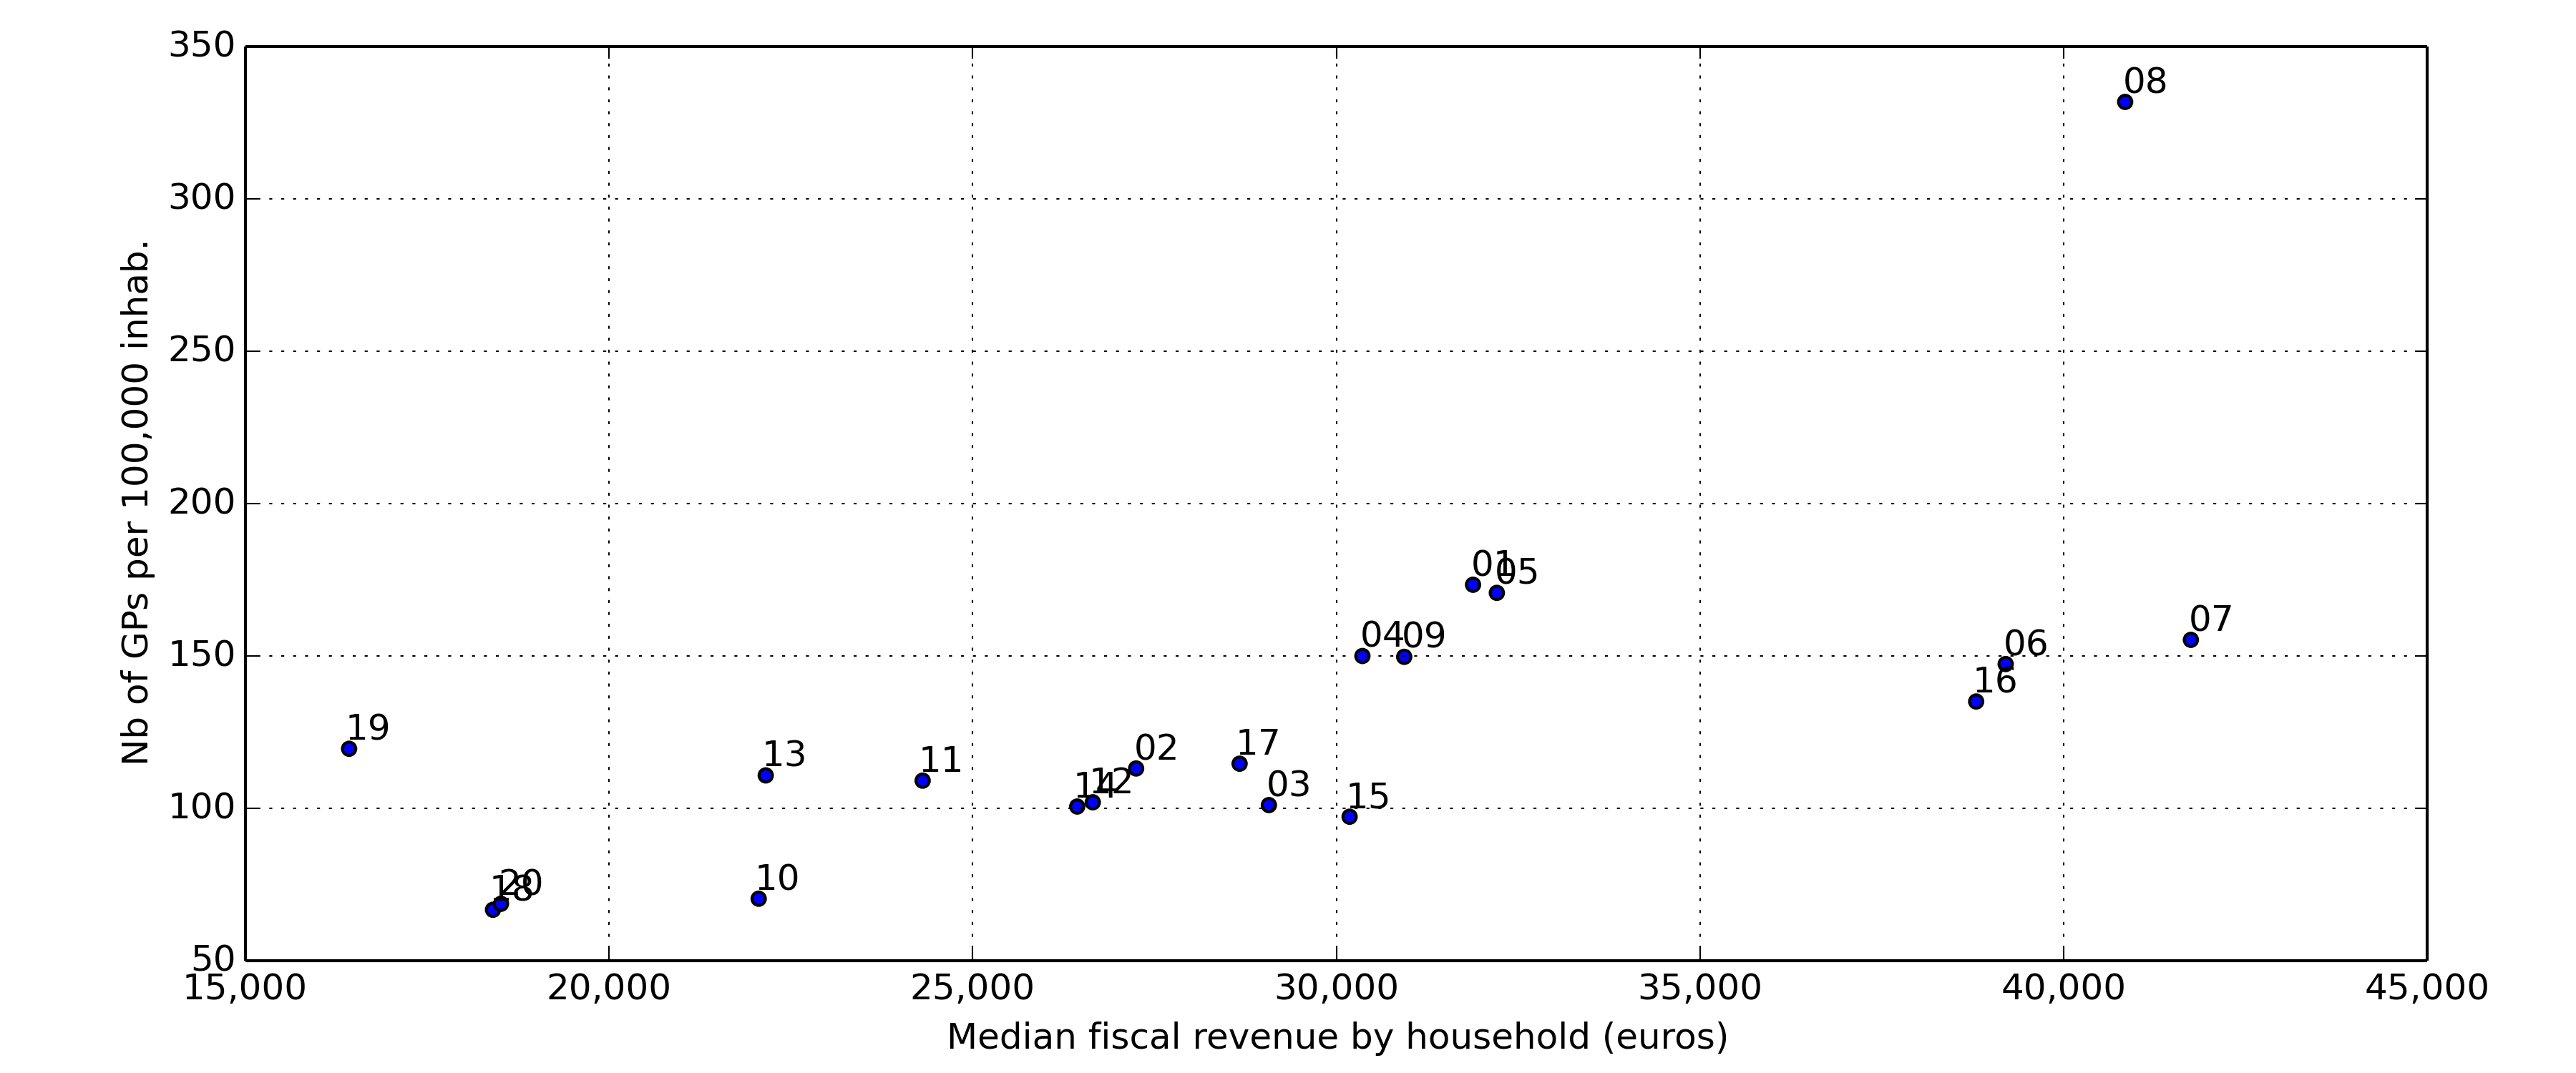
\includegraphics[width=16cm]{images/GP_Ardt_DensityVsRevenue.png}
\end{figure}

\begin{figure}[H]
    \caption{Density of sector 1 GPs vs. household revenue by district}
	\centering
		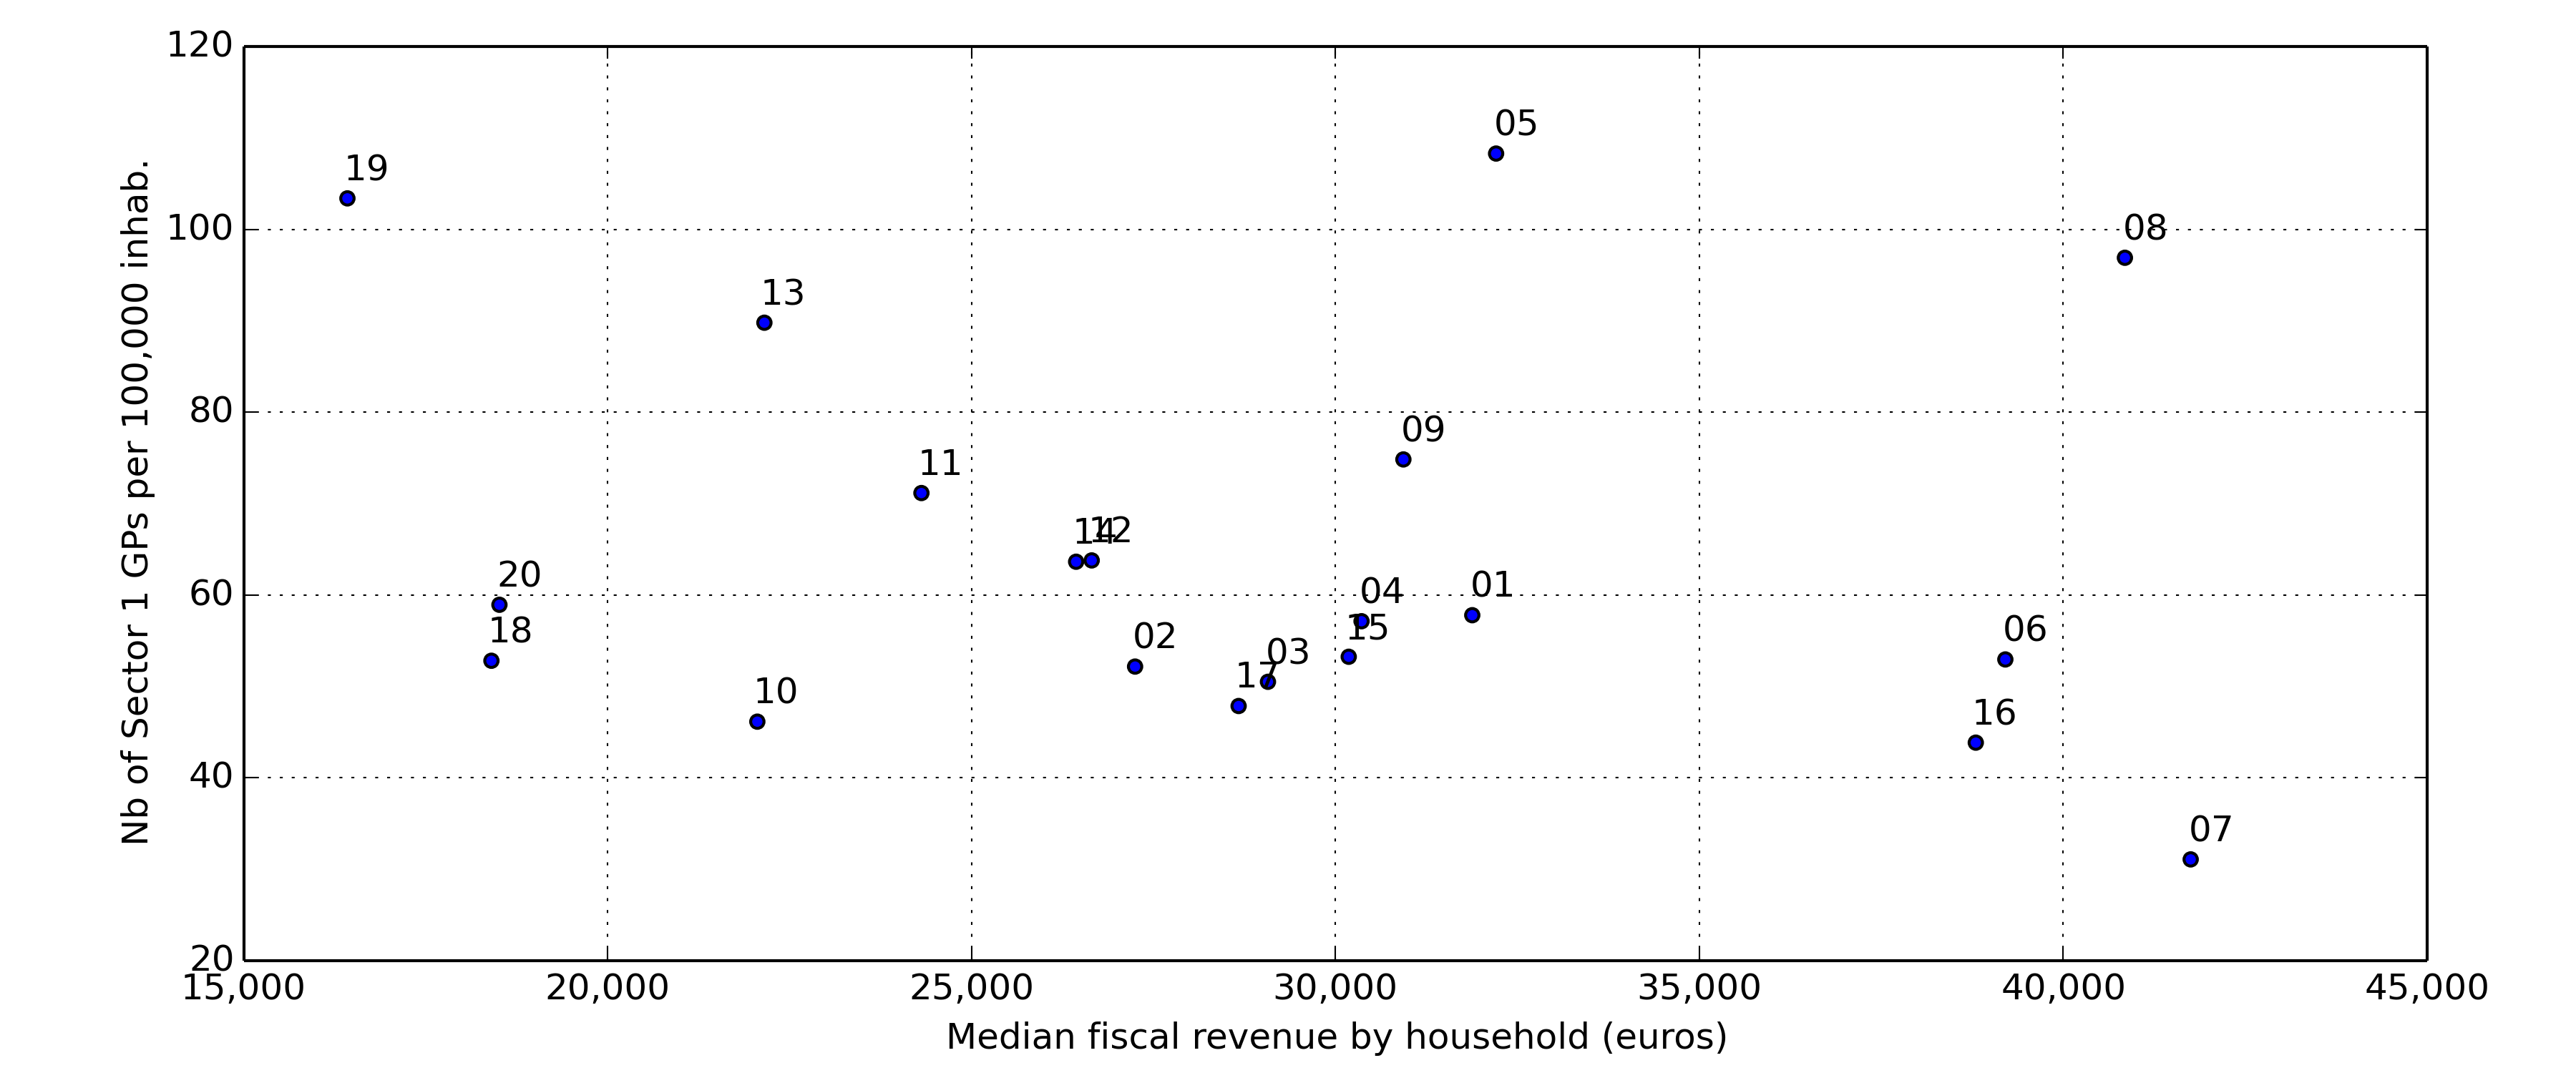
\includegraphics[width=16cm]{images/GP_Ardt_DensityS1VsRevenue.png}
\end{figure}

\begin{figure}[H]
    \caption{Density of sector 2 GPs vs. household revenue by district}
	\centering
		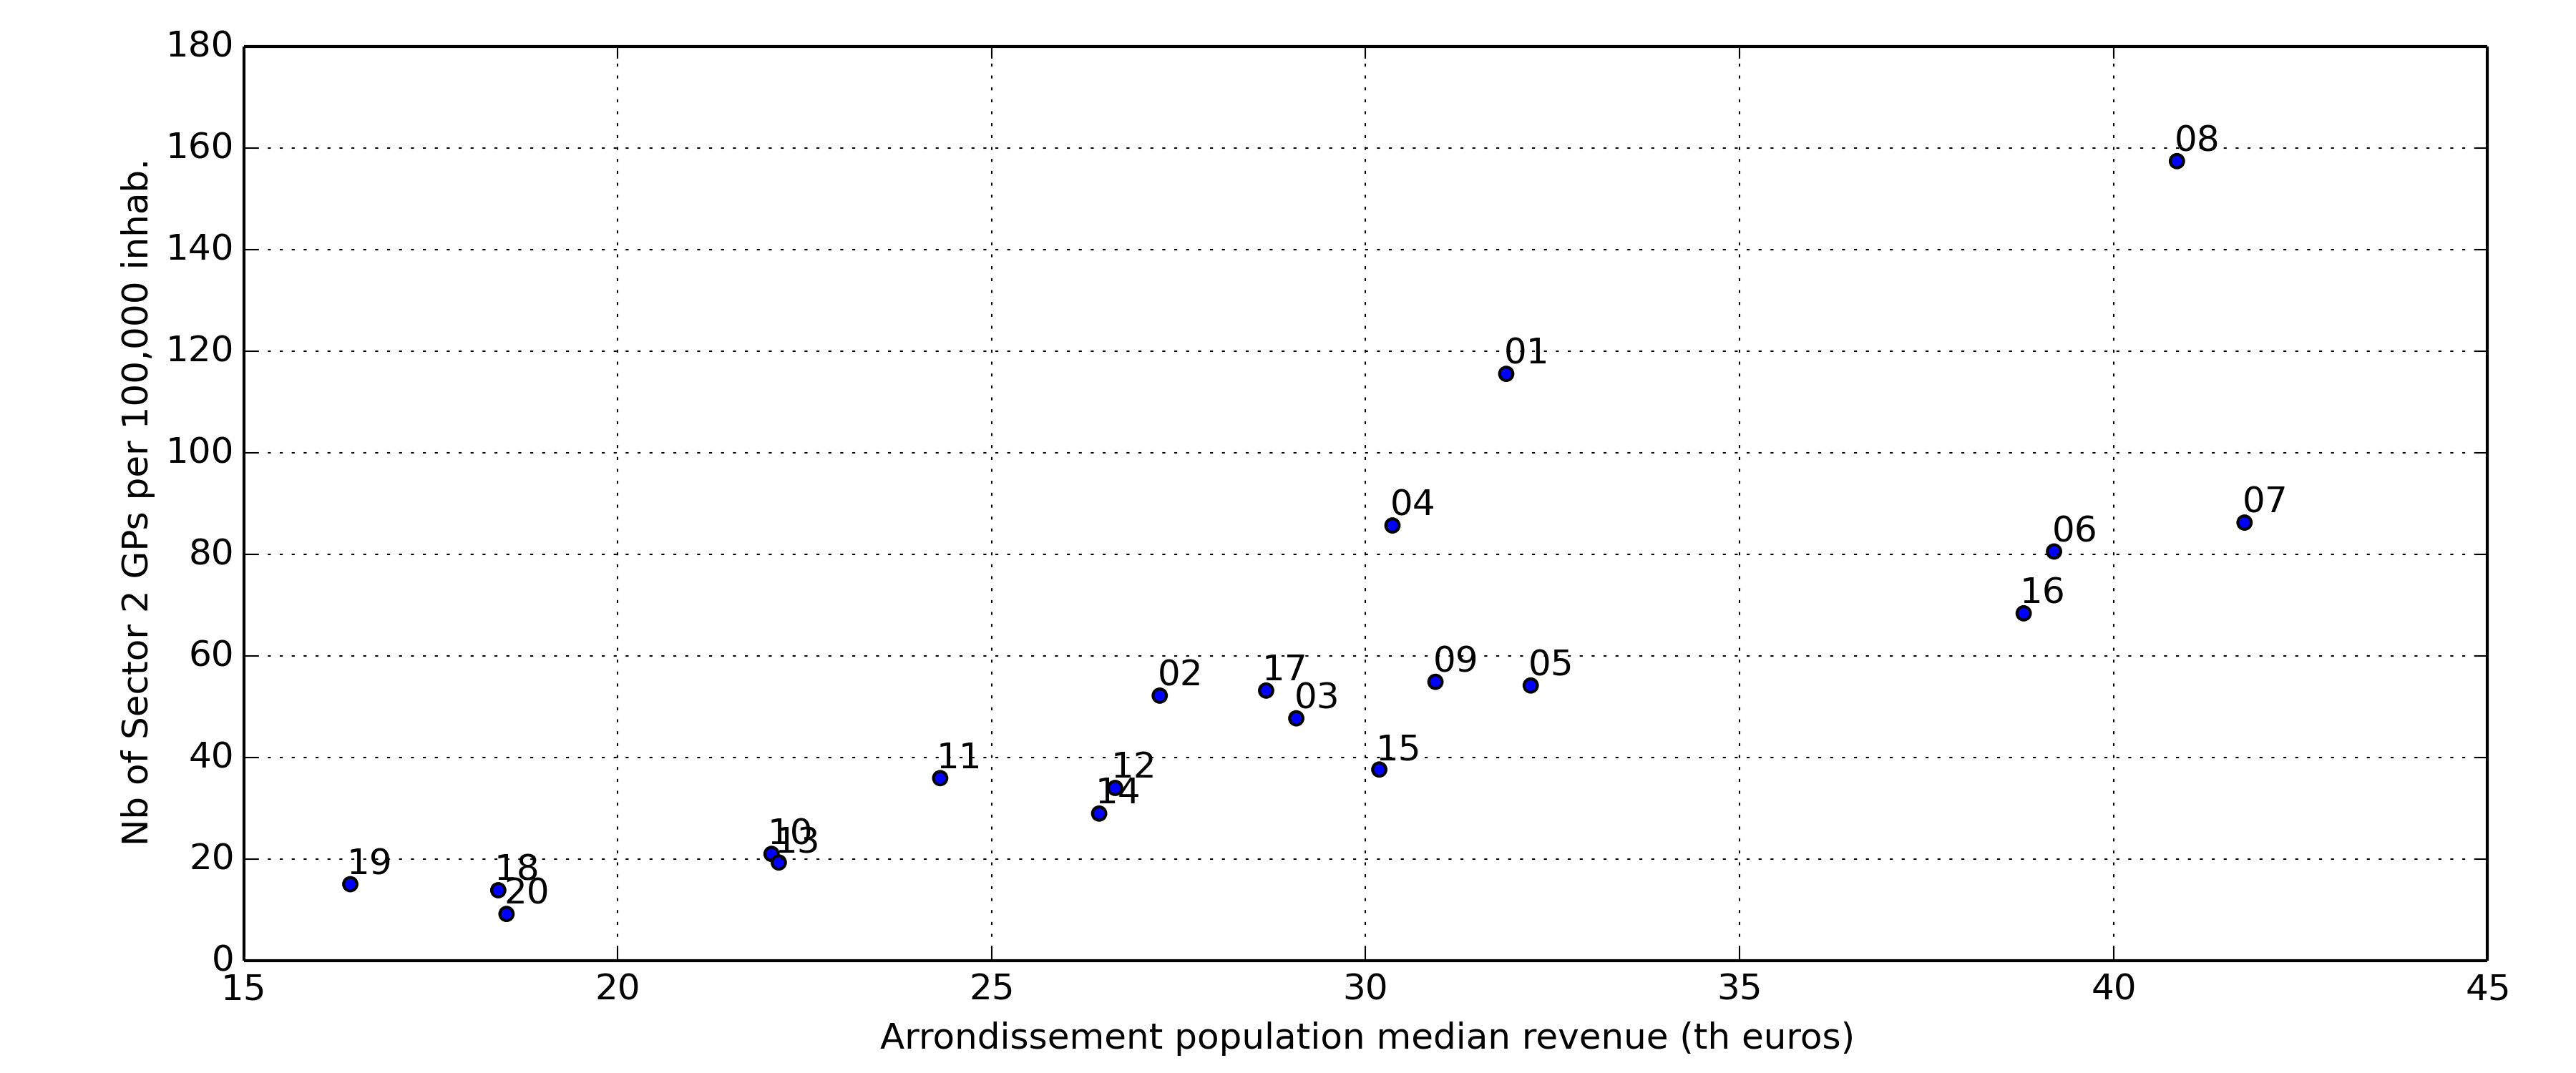
\includegraphics[width=16cm]{images/GP_Ardt_DensityS2VsRevenue.png}
\end{figure}

\begin{figure}[H]
    \caption{Average sector 2 GP consultation price vs. household revenue by district}
	\centering
		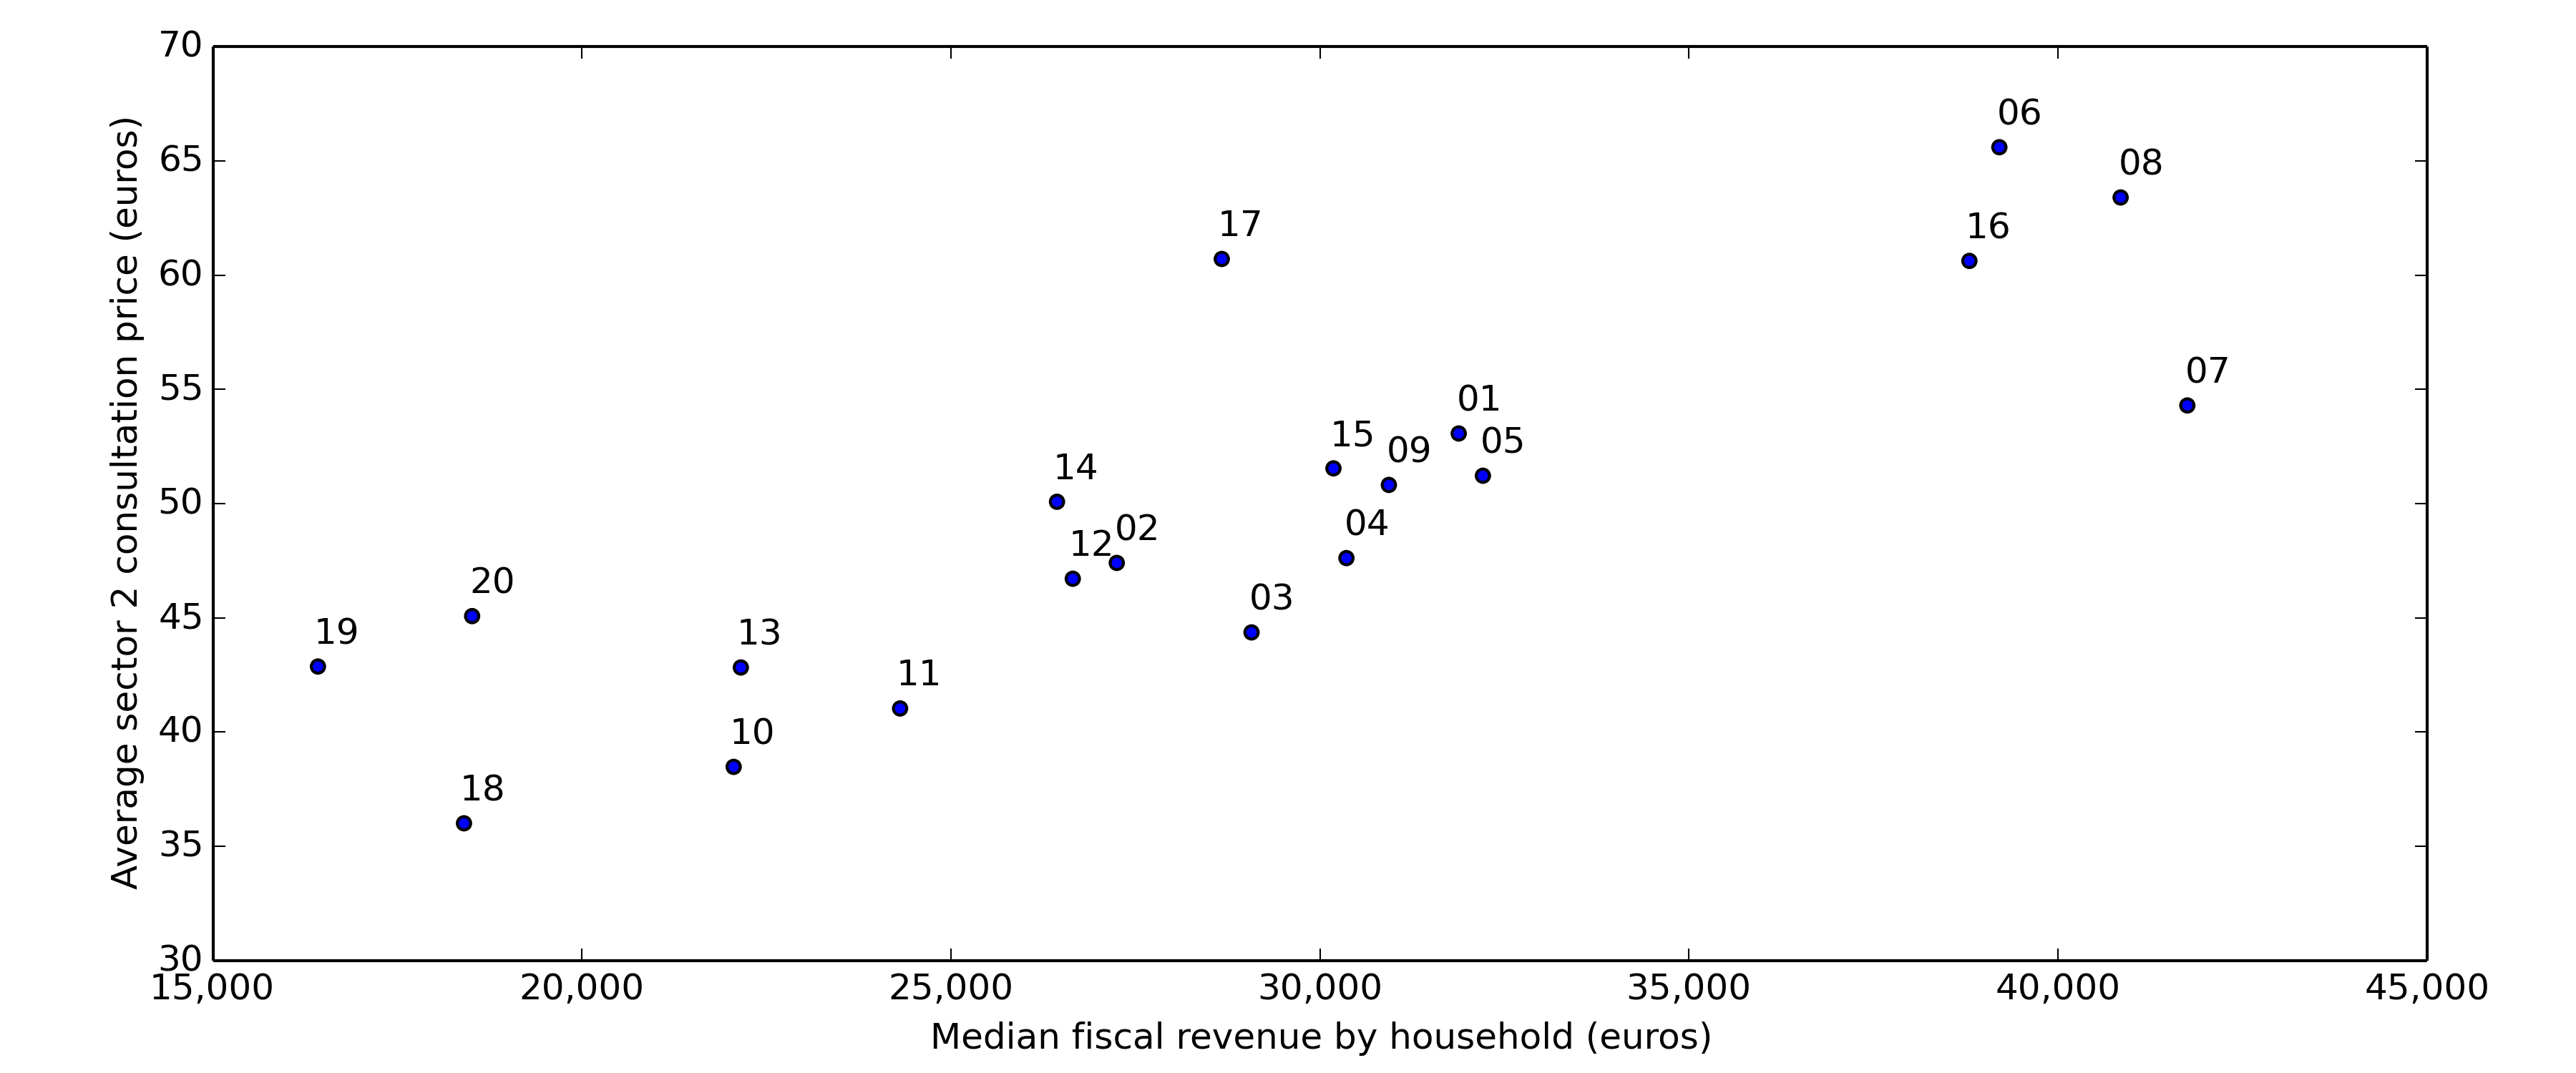
\includegraphics[width=16cm]{images/GP_Ardt_ConsultationS2VsRevenue.png}
\end{figure}

\section{Ophthalmologists}

The number of Ophthalmologists per inhabitant exhibits stronger correlation with revenue than in the case of GPs. The density of sector 1 ophthalmologists is relatively stable across districts, but these account for a small portion of ophthalmologists in Paris. Both the density of sector 2 ophthalmologists and their average consultation price are largely correlated with revenue.

\begin{figure}[H]
    \caption{Density ophtalmologists vs. household revenue by district}
	\centering
		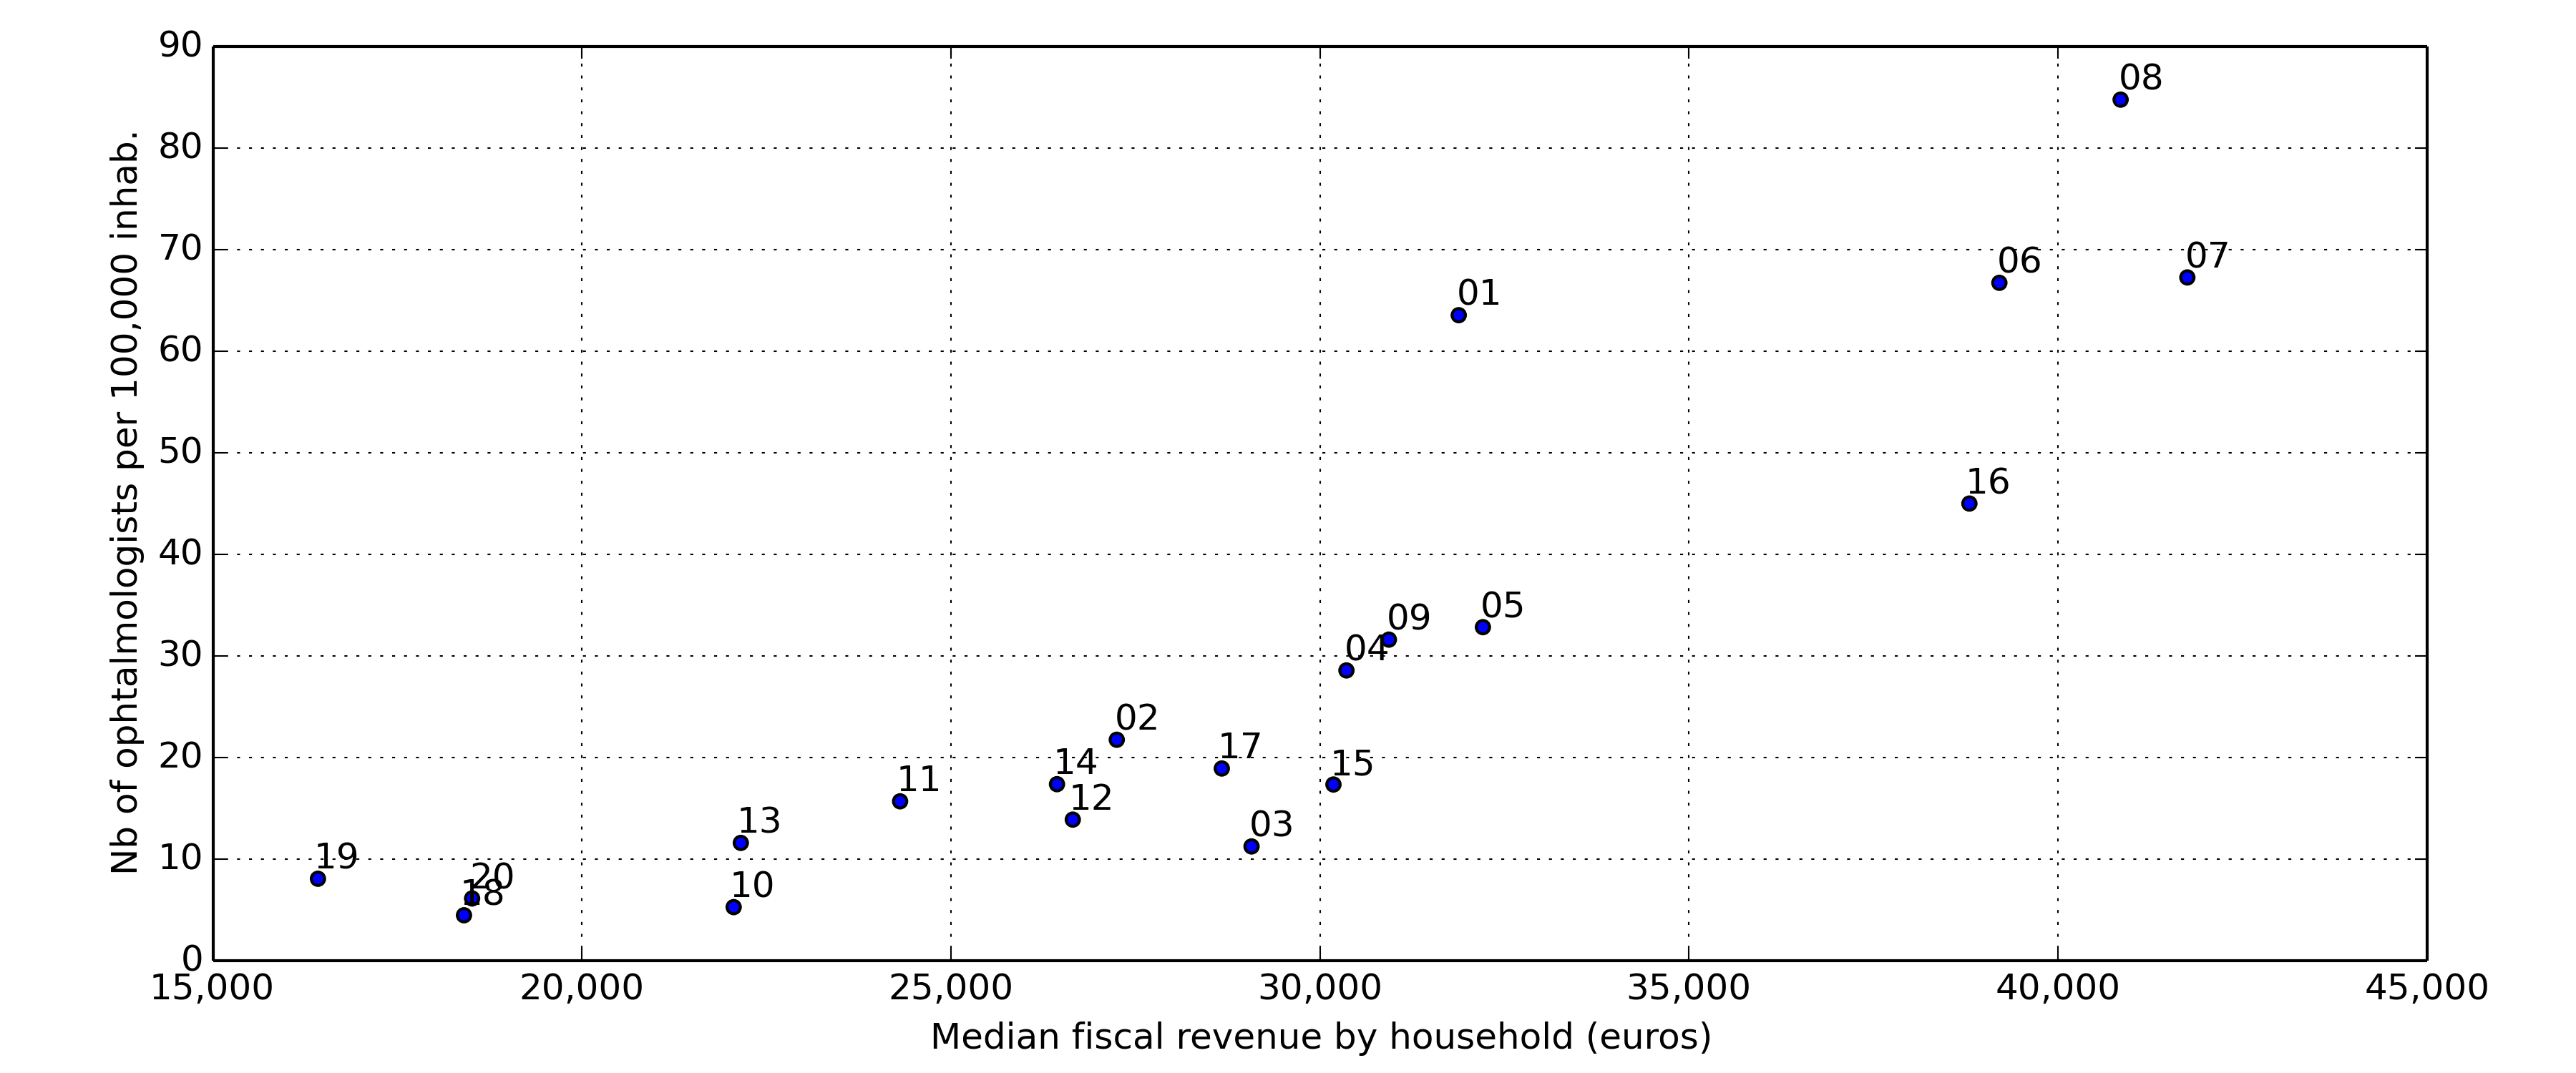
\includegraphics[width=16cm]{images/Ophtalmo_Ardt_DensityVsRevenue.png}
\end{figure}

\begin{figure}[H]
    \caption{Density of sector 1 ophtalmologists vs. household revenue by district}
	\centering
		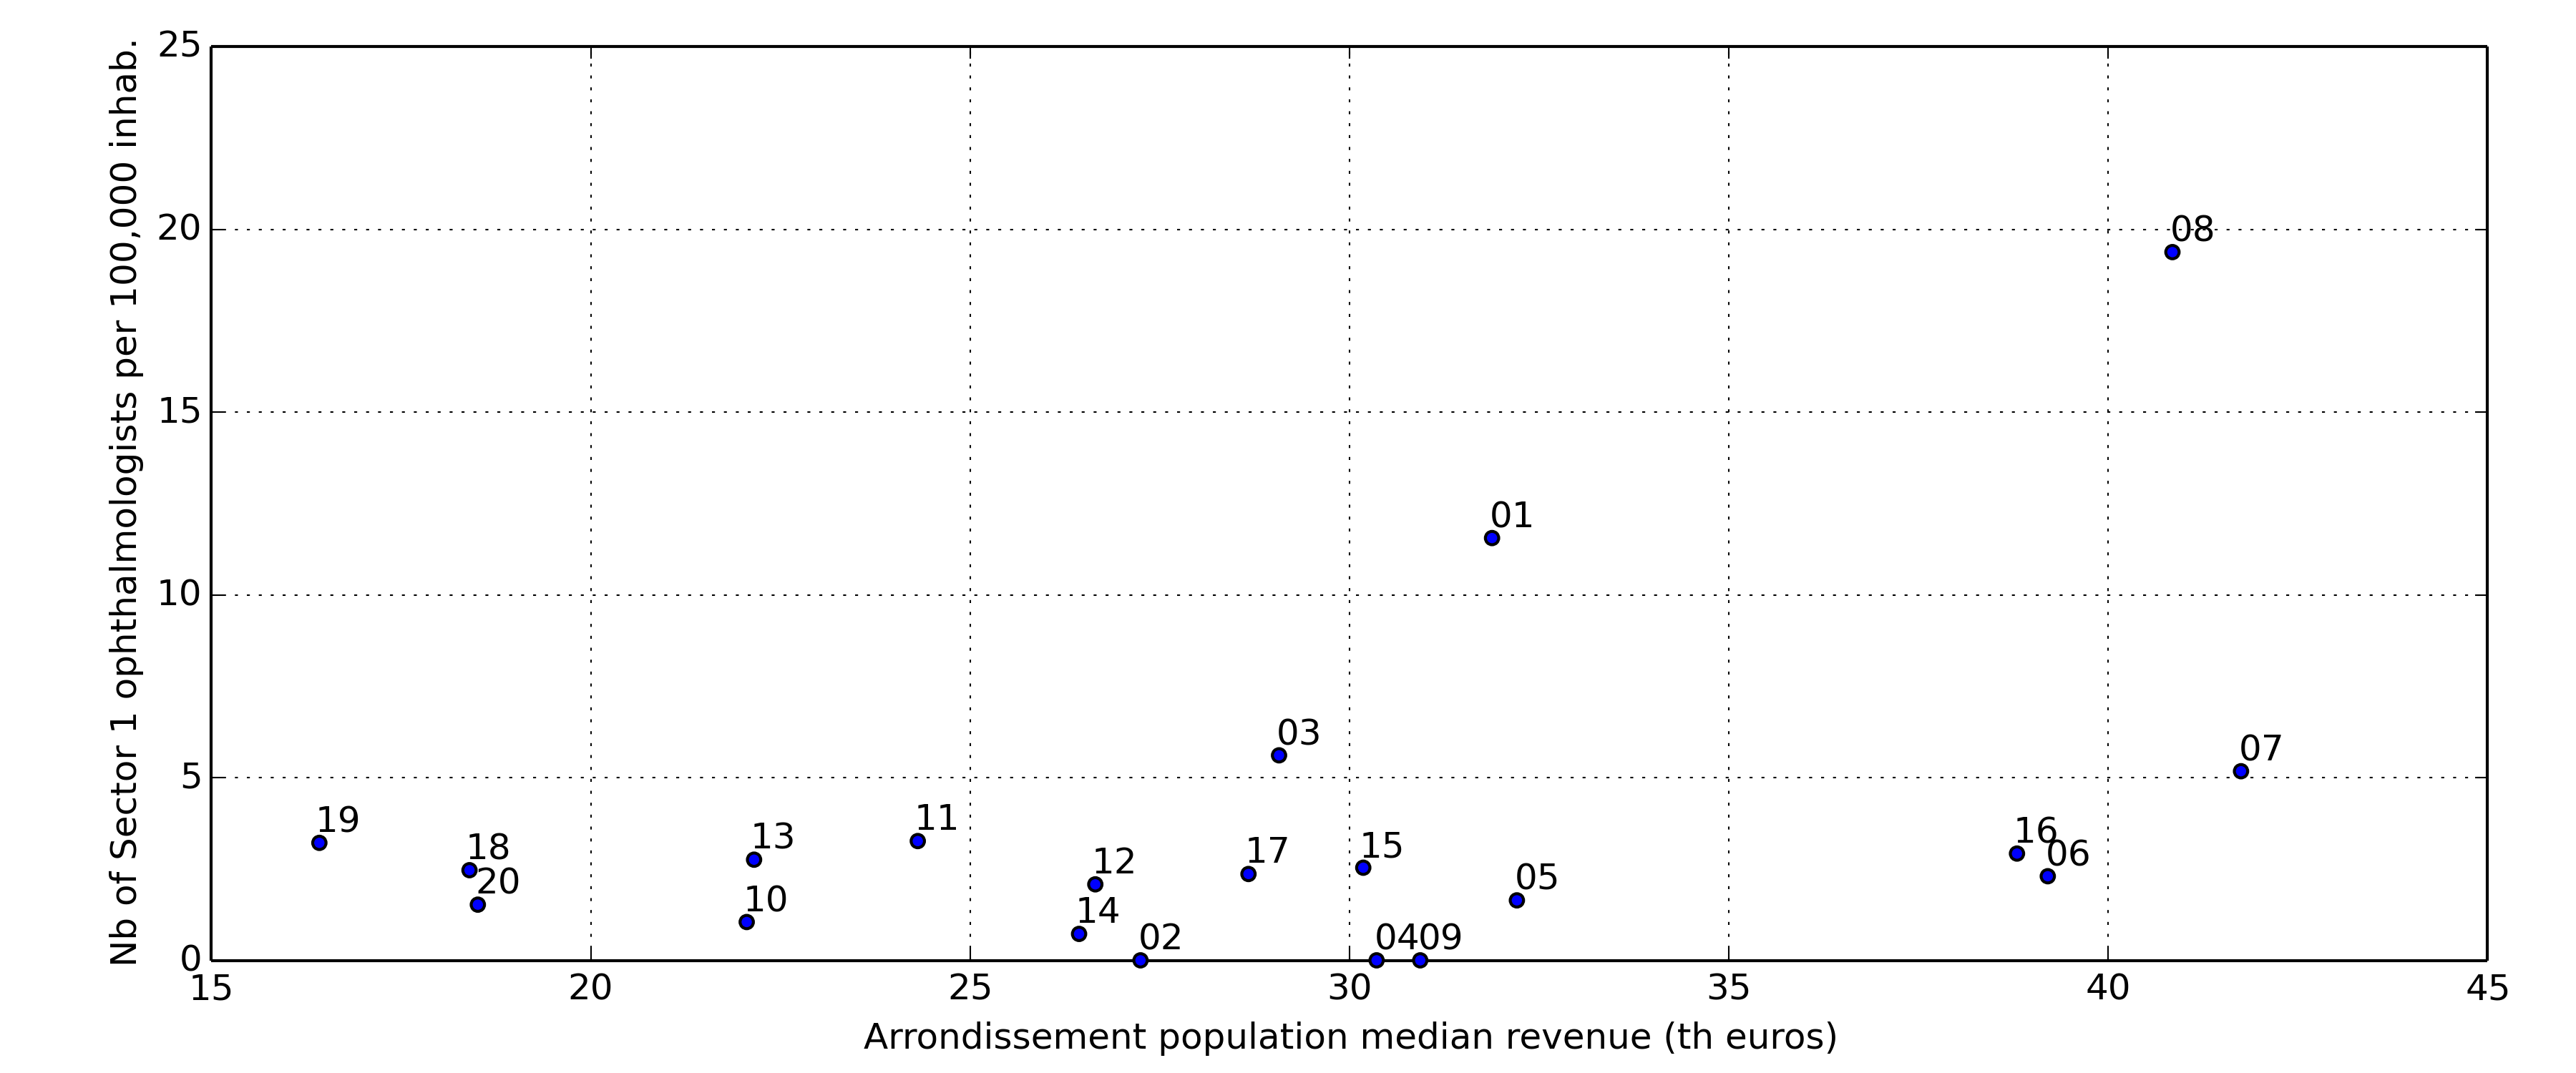
\includegraphics[width=16cm]{images/Ophtalmo_Ardt_DensityS1VsRevenue.png}
\end{figure}


\begin{figure}[H]
    \caption{Density of sector 2 ophtalmologists vs. household revenue by district}
	\centering
		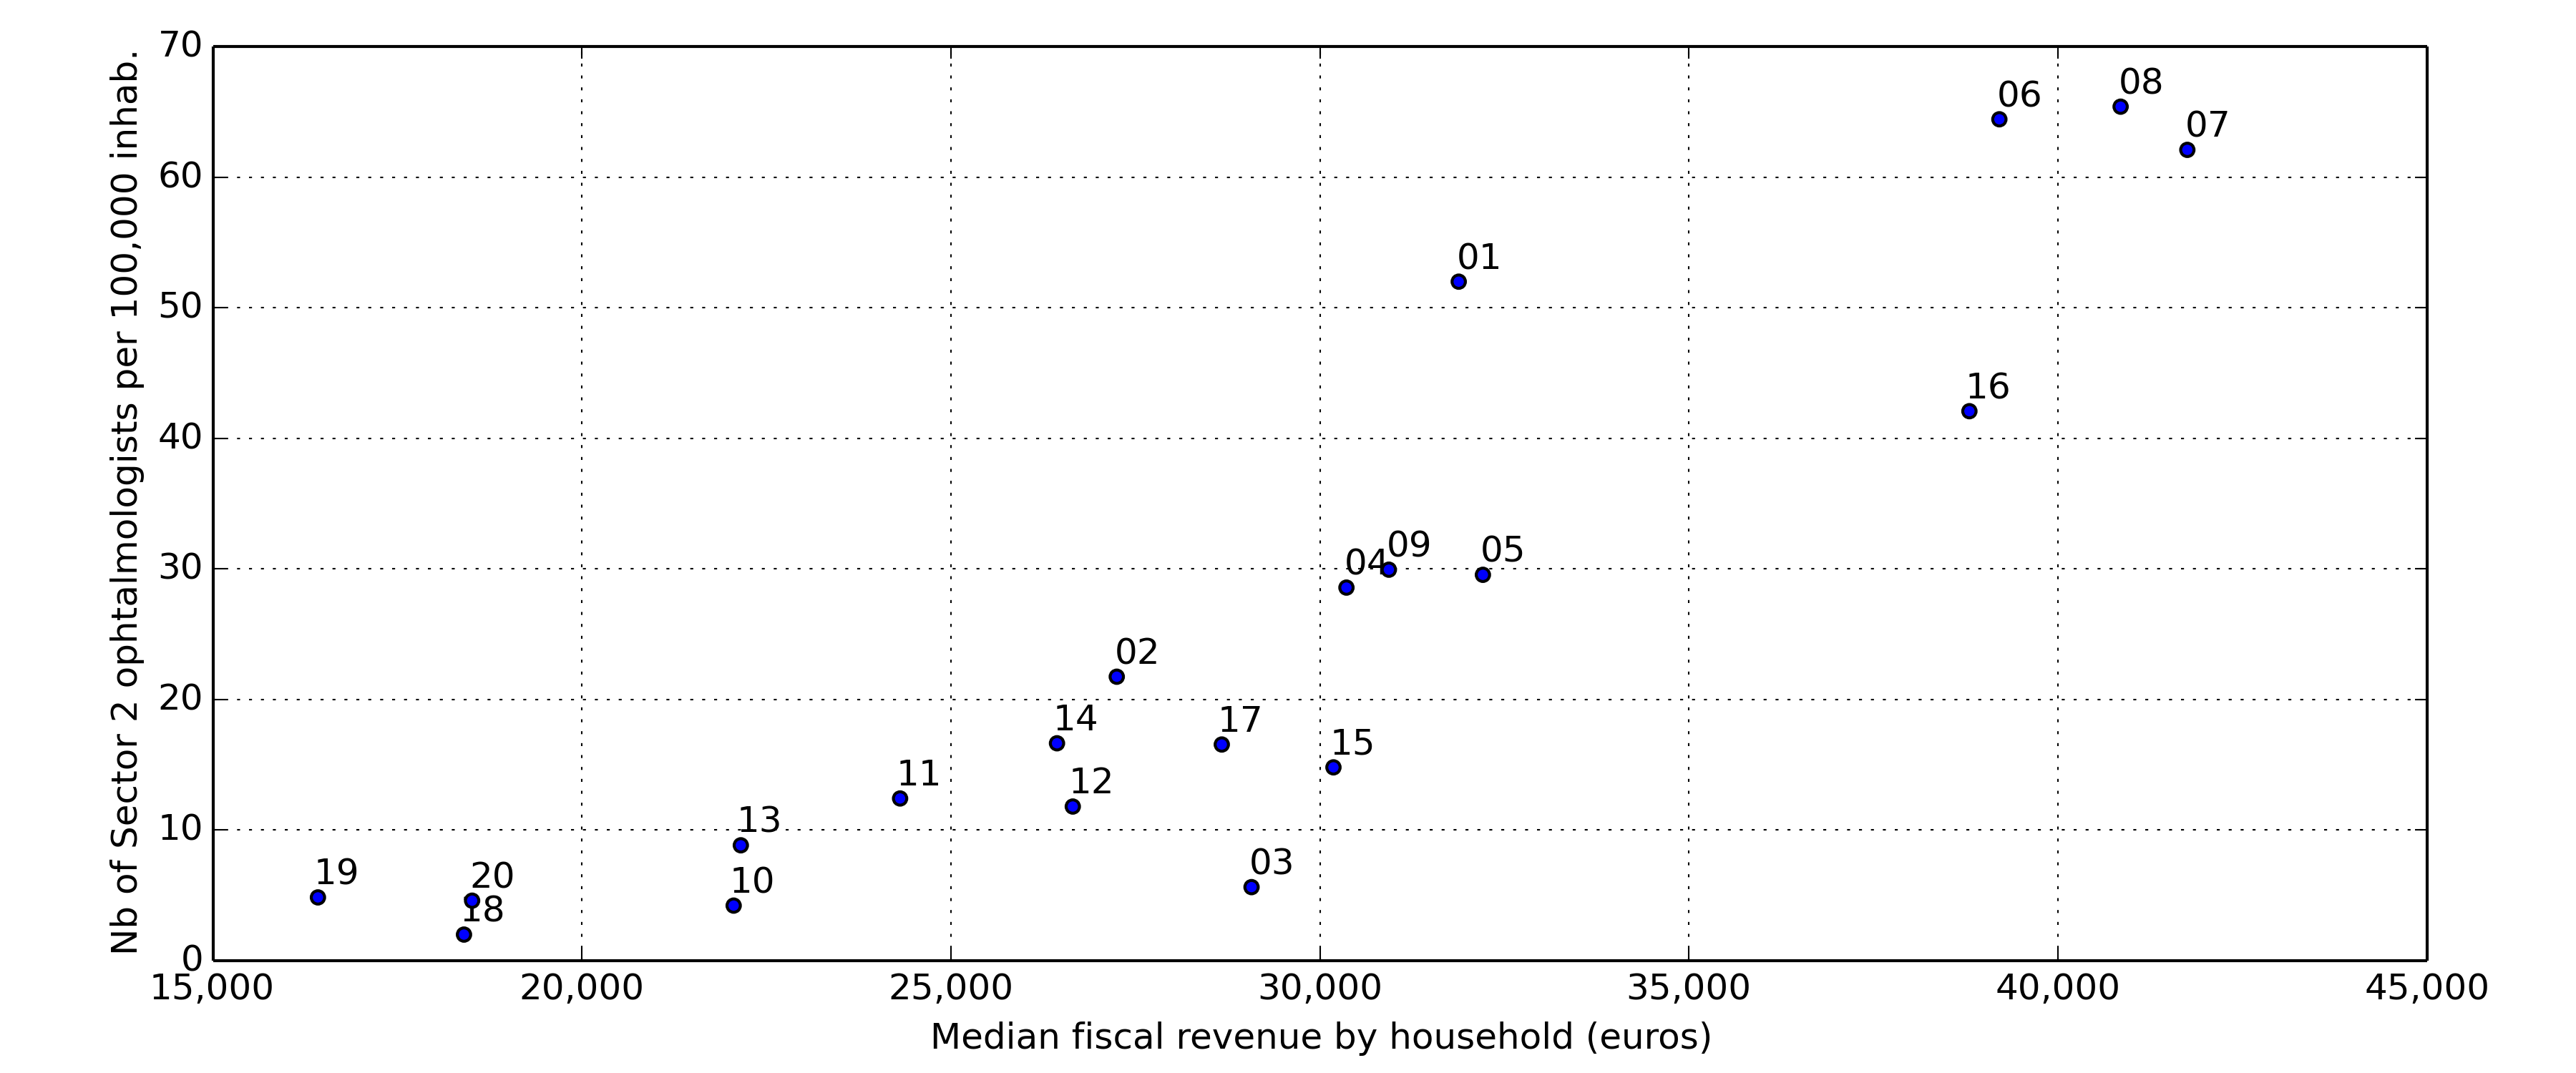
\includegraphics[width=16cm]{images/Ophtalmo_Ardt_DensityS2VsRevenue.png}
\end{figure}

\begin{figure}[H]
    \caption{Average sector 2 ophtalmologist consultation price vs. household revenue by district}
	\centering
		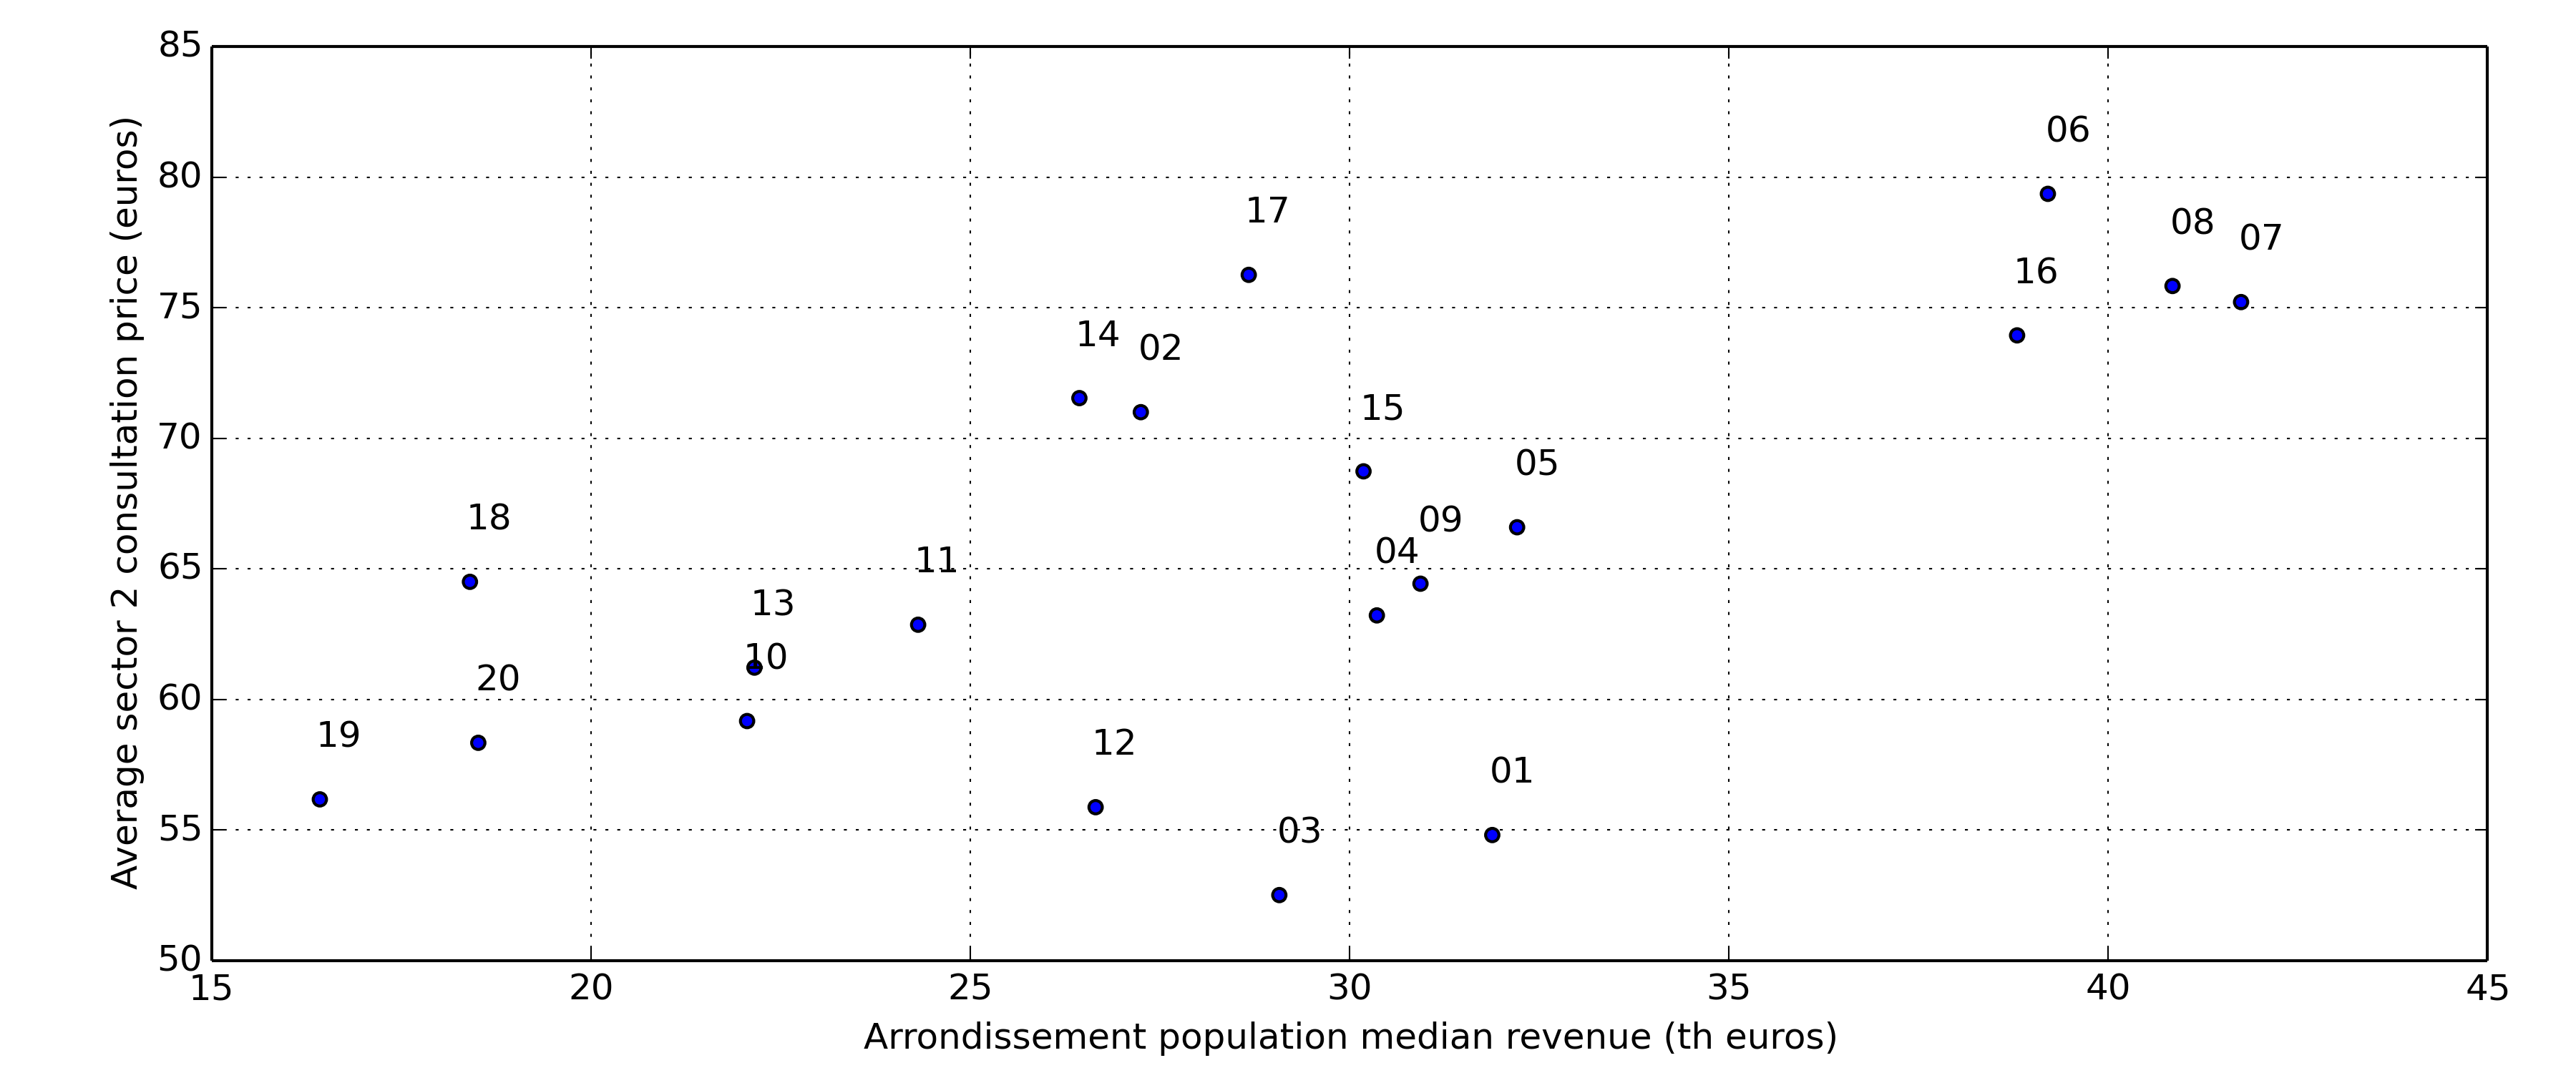
\includegraphics[width=16cm]{images/Ophtalmo_Ardt_ConsultationS2VsRevenue.png}
\end{figure}

\clearpage

\appendix


\end{document}
